\input{free-speech-ott}

\renewcommand{\FSdrulename}[1]{\textsc{\scriptsize #1}}

\newcommand{\tvdash}[1]{\vdash^{#1}}
\newcommand{\arrowT}[5]{(#1 :^{#2} #3)^{#4} \to #5}
\newcommand{\rec}[3]{rec\ #1\ #2\ #3}
\newcommand{\recc}[3]{rec^{-}\ #1\ #3}

The requirement that every program must terminate can be relaxed by
first designing a very powerful programming language (PL), and then
carving out two fragments of programs. The first consists of all the
terminating programs called the logical fragment, and the second
consists of all programs, and this is called the programmatic
fragment. That is we have a picture that looks something like:
\begin{center}
  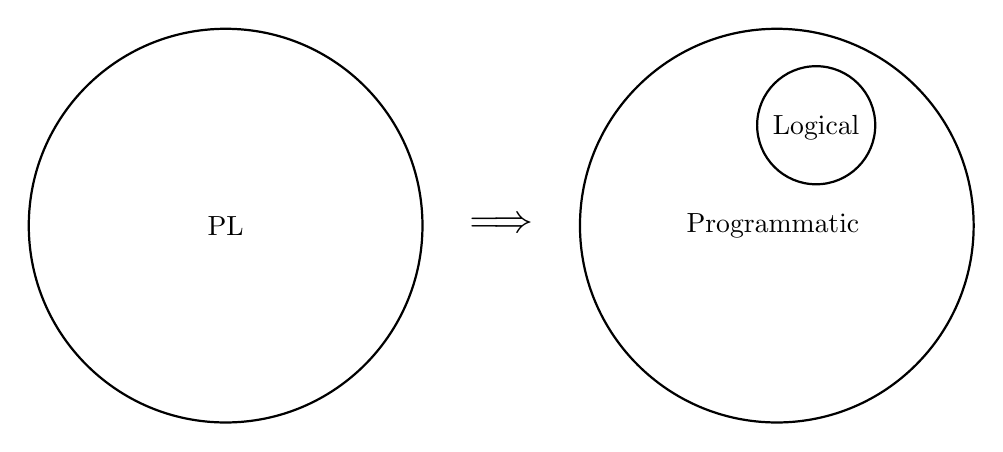
\begin{tikzpicture}[scale=2.5,cap=round,>=latex]
    % draw the unit circle
    \draw[thick] (0cm,0cm) circle(1cm);
    \draw (0cm,0cm) node {PL};
    \draw (1.4cm,0cm) node {\Large $\Longrightarrow$};
    \draw[thick] (2.8cm,0cm) circle(1cm);
    \draw (2.78cm,0cm) node {Programmatic};
    \draw[thick] (3cm,0.51cm) circle(0.3cm);
    \draw (3cm,0.5cm) node {Logical};
  \end{tikzpicture}
\end{center}
The logical fragment will then be considered the ``logical framework''
of the language, and this is where the programs are proofs and the
types are propositions, that is the logical fragment makes use of the
computational trinity (Chapter~\ref{chap:the_three_perspectives}).
Now the programmatic fragment is where all the usual programming will
take place, then one can use the logical fragment to verify properties
of the programs written in the programmatic fragment.  Alternately,
one can understand the fragments as worlds in the sense of possible
world semantics of modal logics.  Below we will see how these two
worlds are connected.  A programming language such as this will need
some additional features to make this all work.

Once the logical fragment has been identified three additional
features will need to be added.  The first feature is that types in
the logical fragment will need to be able to depend on programs from
the programmatic fragment, but this feature has to be designed so as
to prevent these programs from being applied to any arguments or this
would prevent the logical fragment from being logically consistent.
For an overview of logical consistency and how it can be proven see
Chapter~\ref{chap:metatheory_of_programming_languages}.  We call this
feature freedom of speech, because it intuitively states that logical
types and programs can talk about potentially non-terminating
programs, but they are never allowed to actually run them.

The second and third features are usability features.  The logical
fragment is purely specificational.  Its primary use is for the
verification of programs written in the programmatic fragment.
Furthermore, carrying around non-computationally interesting proofs is
expensive.  Thus, it is important to allow some specificational data
to be stripped away during compile time.  In addition, it is important
that the programmer be the one to decide which data is removed.  Now
logical programs are proofs, but they are also terminating programs,
and thus can be considered both logical programs and programmatic
programs.  The third and final feature is the ability to write
programs in the logical fragment and then move them into the
programmatic fragment.  This facilitates code reuse and provides a
means to write verified terminating programs.  We mentioned that the
logical and programmatic fragments can be consider worlds.  Now the
freedom of speech property relates the programmatic fragment to the
logical fragment by allowing the objects of the logical fragment to
express properties about the objects of the programmatic fragment.
Additionally, the feature allowing the programs of the logical
fragment to be moved into the programmatic fragment relates the
logical fragment to the programmatic fragment.  Thus, we have a
situation best captured by the following picture:
\begin{center}
  \begin{tikzpicture}[>=stealth',shorten >=1pt,auto,node distance=5 cm, scale = 1, transform shape]
    \node[state, minimum size=83.1pt] (A)              {Logical};
    \node[state] (B) [right of=A] {Programmatic};
    \node[draw=none] at (9,0) {\large *};

    \path[->] (A) edge [bend left] (B)
              (B) edge [bend left] (A);
  \end{tikzpicture}    
\end{center}
In this chapter we introduce the design of a programming language that
contains all of these features, and some additional ones.  It is
called Freedom of Speech, because it is the first core
dependently-typed functional programming language with the freedom of
speech property.

\section{Syntax and Reduction Relation}
\label{sec:syntax_and_reduction_relation}
We begin by first defining the syntax and reduction relation, and then
move on to the type system.  The features discussed in the
introduction to this chapter will be made explicit when we introduce
the type system, but we will see hints of them in the syntax.

The syntax and the CBV reduction relation is defined in
Figure~\ref{fig:FS-syn-red}.
\begin{figure}
  \begin{center}
    \begin{tabular}{lll}
      Syntax:
      \vspace{10px} \\
      \begin{math}
        \arraycolsep=2pt\edef\arraystretch{1.2}
        \begin{array}{rllllllllllllllll}
          \text{(Classifiers)}  & [[th]] & ::= & [[L]]\,|\,[[C]]\\
          \text{(Stages)}       & [[ep]] & ::= & [[+]]\,|\,[[-]]\\
          \text{(Expressions)}  & [[e]]  & ::= & 
          [[Type]]\,|\,[[Nat]]\,|\,[[x]]\,|\,[[(x : th e1) ep -> e2]]\,|\,[[e1 = e2]]\,|\,
          [[S]]\,|\,[[Z]]\,|\,\\
          & & & [[\x.e]]\,|\,[[rec f x e]]\,|\,[[rec - f e]]\,|\,[[e1 e2]]\,|\,
                [[join]]\,|\,[[injdom]]\,|\,[[injran]]\,|\,\\
          & & & [[contra]]\,|\,[[abort]]\\
          \text{(Values)}       & [[v]] & ::= & 
          [[x]]\,|\,[[Type]]\,|\,[[Nat]]\,|\,[[(x : th v1) ep -> v2]]\,|\,
          [[e1 = e2]]\,|\,[[\x.e]]\,|\,\\
          & & & [[join]]\,|\,[[injdom]]\,|\,[[injran]]\,|\,[[rec f x v]]\,|\,[[rec - f v]]\\
          \text{(Evaluation Contexts)} & [[C]] & ::= & [[ [] ]]\,|\,[[( x : th C ) ep -> e2]]\,|\,[[( x : th e1 ) ep -> C]]\,|\,[[rec f x C]]\,|\,\\
          & & & [[rec - f C]]\,|\,[[e1 C]]\,|\,[[C v]]\\
          \text{(Typing Contexts)}     & [[G]] & ::= & [[.]]\,|\,[[x : th e]]\,|\,[[G1,G2]]\\        
        \end{array}
      \end{math}\\
      & \\
      CBV reduction:\\
      \small
      \begin{mathpar}
        \FSdruleCbvXXApp{}  \and
        \FSdruleCbvXXRec{}  \and
        \FSdruleRedXXCtxt{} \and
        \FSdruleRedXXAbort{} \and
        \FSdruleComputeJoin{}
      \end{mathpar}
    \end{tabular}
  \end{center}  
  \caption{Syntax and reduction rules for freedom of speech}
  \label{fig:FS-syn-red}
\end{figure}
The syntax is collapsed similarly to the Calculus of Constructions --
see Chapter~\ref{sec:the_calculus_of_constructions} for more about the
Calculus of Constructions. So we distinguish between types and terms
(programs) judgmentally.  Expressions and the typing judgment will
depend on two annotations.  The first is called the consistency
classifier and is denoted $[[th]]$ which can be one of $[[L]]$ or
$[[C]]$ where an expression tagged with the former is interpreted to
mean ``belonging to the logical fragment'' and the latter to mean
``belonging to the programmatic fragment.''  The second annotation is
denoted $[[ep]]$ which is called the stage annotation and can be
either $[[+]]$ or $[[-]]$ where the former means ``run time'' and the
latter means ``compile time.'' The consistency classifier essentially
is how we carve out the logical fragment from the programmatic
fragment, and the stage annotation implements the second feature above
where all programs marked as compile time will be erased before run
time.  We now give a brief overview of the syntax of Freedom of
Speech.

Expressions denoted $[[e]]$,$[[e_1]],\ldots,[[e_i]]$ consist of
$[[Type]]$ which is the type of all types, $[[Nat]]$ the type of
natural numbers, variables denoted $[[x]]$,$[[y]]$,$[[z]]$, $\ldots$,
dependent function types denoted $[[(x : th e1) ep -> e2]]$ -- note that
the programmer gets to decide whether an argument is ``logical'' or
``programmatic'' and ``run time'' or ``compile time'' -- next we have
equations denoted $[[e1 = e2]]$, the successor function and the
natural number zero denoted $[[S]]$ and $[[Z]]$ respectively,
$\lambda$-abstractions denoted $[[\x.e]]$, two recursors $[[rec f x
e]]$ and $[[rec - f e]]$ where $[[x]]$ is considered bound in $[[e]]$
in the former, application denoted $[[e1 e2]]$, three forms of proofs
of equations denoted $[[join]]$, $[[injdom]]$, and $[[injran]]$, where
the latter two are injectivity proofs and are discussed further below,
and finally we have two forms of contradictions one logical and one
programmatic denoted $[[contra]]$ and $[[abort]]$ respectively.

The CBV reduction relation is broken up into three different
judgments.  The first is denoted $[[e1 ~b> e2]]$ and defines standard
CBV $\beta$-reduction and consists of two rules
$\FSdrulename{CBV\_App}$ and $\FSdrulename{CBV\_Rec}$ where values are
defined in Figure~\ref{fig:FS-syn-red}.  We will see that the latter rule
can be used for both terminating and non-terminating recursion
depending on which fragment the recursor is typed in.  Note that there
are no congruence rules in the definition of the first judgment.  The
second judgment denoted $[[e1 ~> e2]]$ extends the first with
congruence rules, and a rule for aborting a contradictory computation.
This judgment consists of two rules $\FSdrulename{Red\_Ctxt}$ and
$\FSdrulename{Red\_Abort}$.  These two are defined in terms of
evaluation contexts which can be thought of as a means of specifying
where with in an expression computation can take place. The syntax of
evaluation contexts can be found in Figure~\ref{fig:FS-syn-red}.  This
defines a fragment of the syntax of expressions where exactly one well
formed subexpression has been replaced with a hole.  Holes are denoted
$[[ [] ]]$. Lets consider a few examples:
\begin{example}
  \label{ex:FS-WF-ECTX}
  The following are all well-formed contexts:
  \begin{center}
    $[[((\x.S x) []) ]]$, $[[ ([] Z)]]$, and $[[rec f x (rec g y [])]]$.
  \end{center}
  Now $(\lambda x.[[S]]\,[[ [] ]])\,[[Z]]$ and $[[ [] ]]\,[[ [] ]]$
  are not well-formed contexts.
\end{example}
\noindent
In addition to the syntax of evaluation contexts we also define an
operation that takes an evaluation context and an expression and
``plugs'' the expression into the hole of the context.  

\begin{definition}
  \label{def:FS-ectx-plug}
  Plugging an expression $[[e]]$ into an evaluation context $[[C]]$ is denoted $[[C[e] ]]$
  and is defined by recursion on the form of $[[C]]$ as follows:
  \begin{center}
    \begin{math}
      \begin{array}{rll}
        [[ [] [e] ]]                    & = & e\\
        [[(( x : th C ) ep -> e2)[e] ]] & = & [[( x : th C[e] ) ep -> e2]]\\
        [[(( x : th e1 ) ep -> C)[e] ]] & = & [[( x : th e1 ) ep -> (C[e]) ]]\\
        [[(rec f x C)[e] ]]             & = & [[rec f x (C[e]) ]]\\
        [[(rec - f C)[e] ]]             & = & [[rec - f (C[e]) ]]\\
        [[(e1 C)[e] ]]                  & = & [[e1 (C[e]) ]]\\
        [[(C v)[e] ]]                   & = & [[(C[e]) v]]\\
      \end{array}
    \end{math}
  \end{center}
\end{definition}
At this point one can easily see that the $\FSdrulename{Red\_Ctxt}$
and $\FSdrulename{Red\_Abort}$ are actually a family of congruence
rules parametric in the evaluation context $[[C]]$. Now the rule
$\FSdrulename{Red\_Ctxt}$ simply extended the CBV $\beta$-reduction to
evaluation contexts, while the rule $\FSdrulename{Red\_Abort}$ says
that if $[[abort]]$ appears anywhere in an evaluation context, then the
computation is aborted and concludes just $[[abort]]$.  Lets consider
an example using what we have introduced thus far before moving onto
the type system.

\begin{example}
  \label{ex:FS-syn-red-case}
  First, we define the abstracted booleans and abstracted-boolean case
  similarly to how we defined booleans in system F (see
  Example~\ref{ex:F_terms} in
  Chapter~\ref{chap:the_history_of_type_theory}):
  \begin{center}
    \small
    \begin{math}
      \begin{array}{lll}
        \mathsf{true}     & \defeq [[\x.\f1.\f2.\y.\z.f1 y]]\\
        \mathsf{false}    & \defeq [[\x.\f1.\f2.\y.\z.f2 z]]\\
        \mathsf{case}     & \defeq [[\x.\b.\f1.\f2.\y.\z.(b x f1 f2 y z)]]\\
      \end{array}
    \end{math}
  \end{center}
  We can define the usual Church-encoded booleans in terms of
  abstracted booleans as follows:
  \begin{center}
    \small
    \begin{math}
      \begin{array}{lll}
        \textsf{CH-true}  & \defeq \lambda [[x]].\lambda [[y]].\lambda [[z]].\mathsf{true}\,[[x]]\,([[\x.x]])\,([[\x.x]])\,[[y]]\,[[z]]\\
        \textsf{CH-false} & \defeq \lambda [[x]].\lambda [[y]].\lambda [[z]].\mathsf{false}\,[[x]]\,([[\x.x]])\,([[\x.x]])\,[[y]]\,[[z]]\\
        \textsf{CH-case}  & \defeq \lambda [[x]].\lambda [[b]].\lambda [[y]].\lambda [[z]].\mathsf{case}\,[[x]]\,[[b]]\,([[\x.x]])\,([[\x.x]])\,[[y]]\,[[z]]\\
      \end{array}
    \end{math}
  \end{center}

  Now suppose we have the division $\mathsf{div}$ and the
  $\mathsf{isZero}$ functions.  Then using these we can define a
  function that takes in two natural numbers as input, and then divides
  the first plus two by the second.  However, there is a catch, the
  division function is undefined when the second argument is zero.  So
  instead of leaving the exception handling to the division function
  lets craft our function to throw an error when the second argument
  is zero.  In what way can we throw an error?  This is exactly when
  we use the $[[abort]]$ term.  We can define our function as follows:
  \begin{center}
    \small
    \begin{math}
      \begin{array}{lll}
        \textsf{div-plus-2} & \defeq
        \lambda x.\lambda y.\mathsf{case}\,[[Nat]]\,(\mathsf{isZero}\,y)\,[[(\x.abort)]]\,(\lambda x.(\mathsf{div}\,[[(S (S x))]]\,y))\,y\,x        
      \end{array}
    \end{math}
  \end{center}
  In the definition of the function $\textsf{div-plus-2}$ we had to
  bundle up the abort program inside a constant function to prevent
  our function from always triggering abort.  This insures us that our
  function will abort if and only if it calls the function
  $[[\x.abort]]$.  Similarly, we had to bundle up the division
  function inside a $\lambda$-abstraction so as to insure that it does
  not throw an exception before our function can.  Lets consider some
  computations using $\textsf{div-plus-2}$:
  \begin{center}
    \small
    \begin{tabular}{lll}
      \begin{math}
      \begin{array}{lll}
                 & (\lambda x.\lambda y.\mathsf{case}\,[[Nat]]\,(\mathsf{isZero}\,y)\,[[(\x.abort)]]\,(\lambda x.(\mathsf{div}\,[[(S (S x))]]\,y))\,y\,x)\,[[(S (S Z))]]\,[[Z]] \\
        \redto^2 & \mathsf{case}\,[[Nat]]\,(\mathsf{isZero}\,[[Z]])\,[[(\x.abort)]]\,(\lambda x.(\mathsf{div}\,[[(S (S x))]]\,[[Z]]))\,[[Z]]\,[[(S (S Z))]] \\
        \redto^7 & (\mathsf{isZero}\,[[Z]])\,[[Nat]]\,[[(\x.abort)]]\,(\lambda x.(\mathsf{div}\,[[(S (S x))]]\,[[Z]]))\,[[Z]]\,[[(S (S Z))]] \\
        \redto^* & \mathsf{true}\,[[Nat]]\,[[(\x.abort)]]\,(\lambda x.(\mathsf{div}\,[[(S (S x))]]\,[[Z]]))\,[[Z]]\,[[(S (S Z))]] \\
        \redto^6 & [[(\x.abort)]]\,[[Z]]\\
        \redto   & [[abort]]\\
      \end{array}
    \end{math}\\
    \\
    \begin{math}
      \begin{array}{lll}
                 & (\lambda x.\lambda y.\mathsf{case}\,[[Nat]]\,(\mathsf{isZero}\,y)\,[[(\x.abort)]]\,(\lambda x.(\mathsf{div}\,[[(S (S x))]]\,y))\,y\,x)\,[[(S (S Z))]]\,[[(S (S Z))]] \\
        \redto^2 & \mathsf{case}\,[[Nat]]\,(\mathsf{isZero}\,[[(S (S Z))]])\,[[(\x.abort)]]\,(\lambda x.(\mathsf{div}\,[[(S (S x))]]\,[[(S (S Z))]]))\,[[(S (S Z))]]\,[[(S (S Z))]] \\
        \redto^7 & (\mathsf{isZero}\,[[(S (S Z))]])\,[[Nat]]\,[[(\x.abort)]]\,(\lambda x.(\mathsf{div}\,[[(S (S x))]]\,[[(S (S Z))]]))\,[[(S (S Z))]]\,[[(S (S Z))]] \\
        \redto^* & \mathsf{false}\,[[Nat]]\,[[(\x.abort)]]\,(\lambda x.(\mathsf{div}\,[[(S (S x))]]\,[[S (S Z)]]))\,[[(S (S Z))]]\,[[(S (S Z))]] \\
        \redto^6 & (\lambda x.(\mathsf{div}\,[[(S (S x))]]\,[[S (S Z)]]))\,[[(S (S Z))]]\\
        \redto   & \mathsf{div}\,[[(S (S (S (S Z))))]]\,[[S (S Z)]]\\
        \redto^* & [[S (S Z)]]\\
      \end{array}
    \end{math}
    \end{tabular}
  \end{center}
\end{example}

The previous example illustrates the syntax and the reduction relation
of the freedom of speech language, but it also illustrates how the CBV
reduction order can be manipulated using $\lambda$-abstractions.
Notice that by wrapping the division function up in a
$\lambda$-abstraction we prevent the reduction relation from reducing
it until it is actually needed.  If the $\mathsf{isZero}$ function
returns true then the division function is never needed and thus is
never ran.  This shows how call-by-need reduction can be simulated by
CBV reduction.  

There is one final judgment defined with the reduction relation in
Figure~\ref{fig:FS-syn-red}, and it is denoted $[[e1 \v/ e2]]$. We
call this the joinability judgment and is defined by only one rule
\FSdrulename{ComputeJoin}. This rule stats that whenever there exists
an expression $[[e]]$ such that the expressions $[[e1]]$ and $[[e2]]$
both reduce to $[[e]]$ in any number of steps, then $[[e1]]$ and
$[[e2]]$ are joinable.  If $[[e1 \v/ e2]]$ holds then we consider the
expressions $[[e1]]$ and $[[e2]]$ to be equivalent.  This judgment
will be used to give the $[[join]]$ expression its type in the typing
rule \FSdrulename{join}.
% section syntax_and_reduction_relation (end)

\section{Type System}
\label{sec:type_system}
Throughout this thesis we have seen that the reduction rules paired
with the type system is really where the heart of the programming
language or type theory lives.  The reduction rules tells us how to
compute while the typing rules tell us which programs are valid and
which programs we can consider as proofs.  In this section we present
the typing rules of Freedom of Speech, and we will make explicit how
it contains all of the features we introduced in the introduction to
this chapter.  

The type system contains many rules, and so we break up the system and
introduce it in chunks.  To see the complete definition in one place
see Appendix~\ref{sec:freedom_of_speech_all}.  Recall from the
previous section that the syntax is collapsed.  Types and programs are
described by a single syntactic category called expressions.  This
then implies that we only have a single judgment defining the typing
relation.  This judgment is denoted $[[G |- e : e' th]]$, and we read
this judgment as the expression $[[e]]$ has type $[[e']]$ in fragment
$[[th]]$ in environment $[[G]]$.  We can think of this judgment as
being parametric in $[[th]]$, and thus is two judgments in one.  If
$[[th]]$ is $[[L]]$, then $[[e]]$ is a proof or logical program, while
if $[[th]]$ is $[[C]]$, then $[[e]]$ is a potentially diverging
program.  So it is the typing judgment that does the carving out of
the two fragments.

We begin introducing the type system with the kinding rules:
\begin{center}
  \begin{mathpar}
    \FSdruleKXXType{} \and
    \FSdruleKXXNat{}  \and
    \FSdruleKXXPi{}   \and
    \FSdruleKXXEq{}          
  \end{mathpar}
\end{center}
The expression $[[Type]]$ is a universe containing all of the
expressions that can be considered well-defined types with respect to
an environment.  Hence, we call an expression $[[e]]$ a type if and
only if $[[G |- e : Type th]]$ for some environment $[[G]]$.  If
$[[th]]$ is $[[L]]$, then $[[e]]$ is can be considered a formula
otherwise $[[e]]$ is simply a type.  The rules above tell us that
there are four types: the type $[[Type]]$, which is only a
programmatic type (for the explanation why see
Section~\ref{sec:martin-lofs_type_theory}), the type of natural
numbers, dependent product types, and equations between well typed
expressions.  These are the only expressions that will be considered
types.

A few remarks about the types.  Notice that the rule
$\FSdrulename{K\_Pi}$ does not require the consistency classifier of
the arguments to match the consistency classifier of the range type.
This allows functions to take in arguments from one fragment and then
produce a program of the opposite fragment.  For example, the type
$[[(x : C Nat)+ -> x = x]]$ takes a programmatic argument, but
produces a formula which is the statement that $[[x]]$ is equivalent
to itself.  Thus, formulas can depend on potentially diverging
programs.  This is exactly the freedom of speech property.  Finally,
note that the expressions of an equation do not have to have the same
type.  This is called heterogenous equality.  In addition, note that
the consistency classifiers for the two equations can be different.
For example, $[[S Z]]$ is logical and programmatic, thus $[[S Z = S
Z]]$, where the first is logical and the second is programmatic, is a
valid expression.

Now that we have characterized the types we can introduce how both
logical and programmatic programs are typed.  First, we introduce the
axioms for natural numbers and assumptions:
\begin{center}
  \begin{mathpar}
    \FSdruleSucc{} \and
    \FSdruleZero{} \and
    \FSdruleVar{}  
  \end{mathpar}
\end{center}
The astute reader will have noticed that natural numbers are typed
only in the logical fragment, but one might think that these are
purely programmatic, because they do not make for very interesting
formulas.  As we mentioned above the logical fragment can be
considered as a terminating functional programming language so if one
wishes to insure that the program they are constructing is terminating
then they can construct it in the logical fragment.  To use the
natural numbers in the programmatic fragment we add an additional
typing rule:
\begin{center}
  \begin{mathpar}
    \FSdruleCoerce{}
  \end{mathpar}
\end{center}
This rule allows any well-typed logical expression to be coerced into
the programmatic fragment.  This corresponds to the edge relating the
logical fragment to the programmatic fragment in the diagram * from
the introduction of this chapter.  Thus, natural numbers can be used
in either fragment.  The third rule we introduce above is the variable
rule \FSdrulename{Var} which depends on the premise $[[G |- e : Type
th]]$.  This premise -- we will see these all throughout the
definition of the typing relation -- insures that the expression
$[[e]]$ is indeed a type.  This is necessary because we only have one
syntactic category for expressions, so the only way to tell the
difference between a type and an expression is by using the typing
judgment.

Programmatic and logical functions are introduced using two styles of
$\lambda$-abstractions:
\begin{center}
  \begin{mathpar}
    \FSdruleLam{}       \and
    $$\mprset{flushleft}
    \inferrule* [right=ILam] {
      [[G |- e1 : Type th']]
      \\\\
      [[G, x : th' e1 |- v : e2   th]]
      \\
      [[x notin FV(v)]]
    }{[[G |- v : (x : th' e1) - -> e2 th]]}
  \end{mathpar}
\end{center}
The former introduces $\lambda$-abstractions with runtime relavent
arguments, while the latter introduces $\lambda$-abstractions whose
argument is compile time relavent only.  We call the latter implicit
$\lambda$-abstractions, because the argument is left implicit.  The
\FSdrulename{Lam} rule is intuitive, but notice that again the arguments
consistency classifier does not have to match the bodies, thus
allowing freedom of speech.  

The typing rule \FSdrulename{ILam} has a restriction on the body of
the implicit $\lambda$-abstraction, infact there are a number of value
restrictions in the definition of the typing relation.  This
restriction is necessary in order to maintain the meta-theoretic
property called progress. This property states that every well-typed
program can either take a computational step or is already a value.
Suppose the restirction on \FSdrulename{ILam} is lifted. Then the
judgment $[[. |- Z Z : (x : L Nat = (y : L Nat) + -> Nat)- -> Nat L]]$
holds, but $[[Z Z]]$ is niether a value nor a redex.  It is a stuck term!
Thus, this value restriction is necessary to rule out stuck terms of
this form.

Now we have two distinct $\lambda$-abstractions, and thus we will need
two types of applications:
\begin{center}
  \begin{mathpar}    
    \FSdruleAppPiTerm{} \and
    \FSdruleAppAllTerm{}
  \end{mathpar}
\end{center}
The former eliminates function types with runtime arguments, while the
latter eliminates function types with compile-time arguments.  These
rules are straightforward, but do contain value restrictions similar
to \FSdrulename{ILam}.  These restrictions prevent the application of
a logical function to a diverging non-value computation.  For example,
if we lift the value restriction then we could type
$([[e]]\,\mathsf{loop})$ in the logical fragment, where
$\mathsf{loop}$ is a program that simply calls itself infinitely
often, but then the term $([[e]]\,\mathsf{loop})$ diverges, and hence
is no longer a proof.  Remember, logical programs cannot run
programmatic programs.

So far we have seen the typing rules for types, natural numbers,
$\lambda$-abstractions, and applications.  Now we introduce the typing
rules for introducing and eliminating -- or using -- equations.  The
typing rules are as follows:
\begin{center}
  \begin{mathpar}
    \FSdrulejoin{}       \and
    \FSdruleConv{}       \and    
  \end{mathpar}
\end{center}
The former introduces an equation by first judging that the
expressions $[[e]]$ and $[[e']]$ are joinable as defined in
Figure~\ref{fig:FS-syn-red}, then requiring that $[[e]]$ and $[[e']]$
be well typed.  Note that the expressions $[[e]]$ and $[[e']]$ can
have different types and consistency classifiers.  Thus, this rule
introduces heterogenous equality.  Now equations are completely
logical hence we can consider $[[join]]$ as the proof that $[[e]]$ and
$[[e']]$ are equivalent.  Furthermore, $[[e1]]$ and $[[e2]]$ can be
$[[Type]]$, thus $[[e]]$ and $[[e']]$ can be types making $[[join]]$ a
proof of an equation between types.  We can now introduce equations,
but how are they used?  If we have a proof that the expressions
$[[e1]]$ and $[[e1']]$ are equivalent, that is we know 
$[[G |- e' : e1 = e1' L]]$, and if we also have an expression $[[e]]$ whose
type depends on $[[e1]]$, then the rule \FSdrulename{Conv} allows us to replace
$[[e1]]$ in the type $[[e]]$ with its equivalent $[[e1']]$.  Thus,
the rule \FSdrulename{Conv} allows one to substitute equals for equals in types.

The rules \FSdrulename{Join} and \FSdrulename{Conv} have one
particular disadvantage.  Suppose 
\[ 
  \begin{array}{lll}
    [[G]] \defeq [[z: L Type, y: L Type, x: L z, u: L ((a : L Nat) + -> z) = ((a : L Nat) + -> y)]], \\
    [[G |- \a.x: (a : L Nat) + -> z L]] \text{, and }\\ 
    [[G |- Z : Nat L]].
  \end{array}
\]  Then $[[G |- (\a.x) Z : z L]]$.  By applying $\FSdrulename{Conv}$ and using
the assumption $u$, we may conclude $[[G |- (\a.x) Z : y L]]$, but 
$[[(\a.x) Z ~> x]]$ and $[[G |- x:z L]]$.  Therefore, we have obtained a counterexample to type preservation!
Notice that if we knew $[[z = y]]$ then this would no longer be a counterexample, but it is impossible to prove that $[[z = y]]$
from knowing $[[((a : L Nat) + -> z) = ((a : L Nat) + -> y)]]$ using only \FSdrulename{Join} and \FSdrulename{Conv}.  So
to prevent counterexamples such as these we add the following rules:
\begin{center}  
  \begin{mathpar}
    \FSdruleInjDom{} \and
    \FSdruleInjRan{}
  \end{mathpar}
\end{center}
These rules are known as injectivity rules for dependent products.
The second rule may seem a bit strange, especially the second premise,
because we are substituting a value $[[v]]$ for two free variables of
possibly different types.  This is, however, not a problem, because
from the premises of $\FSdrulename{InjRan}$, $\FSdrulename{InjDom}$,
and $\FSdrulename{Conv}$ we may conclude $[[G |- v:e'1 th]]$.  Then by
$\FSdrulename{InjDom}$ we know $[[G |- injdom:e1 = e'1 L]]$, and
clearly $[[G |- v : e1 th]]$ is equivalent to $[[G |- v : [e1/x]x
th]]$.  Thus by $\FSdrulename{Conv}$, $[[G |- v : [e'_1/x]x th]]$, which
is equivalent to $[[G |- v:e'1 th]]$.  So the rule
\FSdrulename{InjRan} is sound.

Equational reasoning is based on the runtime behavior of programs, but
there a number of different programs of a different type so what
happens when it is possible to obtain a equation between contradicting
values?  The reader may object to the very question, because the
logical fragment -- as we have said above -- must be consistent, but
it is possible to start with inconsistent assumptions, and in these
cases the logical fragment needs to be able to trigger a
contradiction.  We introduce the following rules to eliminate
contradictory equations:
\begin{center}
  \begin{mathpar}
    \FSdruleAbort{}       \and
    \FSdruleContra{}      \and
    \FSdruleContraAbort{}
  \end{mathpar}
\end{center}
The first rule introduces $[[abort]]$ and states that $[[abort]]$ can
have any type.  As we have seen above $[[abort]]$ is used to indicate
error states.  The second rule, \FSdrulename{ContraAbort}, introduces
the proof $[[contra]]$ with any well-defined type as long as there is
a proof of some value being equivalent to $[[abort]]$.  This means, if
a program enters an error state, then a contradiction has occurred. An
example might be trying to verify the correctness of $\mathsf{div}$
for all natural numbers.  Then when $[[Z]]$ is given as the second
argument it will reduce to abort.  Thus, we would be able to obtain
our result by using $[[contra]]$.  The third rule, \FSdrulename{Contra},
is similar to the previous rule, except it requires a proof that
$[[Z]]$ is equivalent to a natural number greater than $[[Z]]$.  

There is one additional type of inconsistent equations that might be
introduced that can cause major problems.  The fact that in an
inconsistent context one can prove two dependent products equivalent
when they have differing stage annotations or consistency classifiers
can break freedom of speech.  For example, it would be possible to
equate programmatic functions taking programmatic arguments to
programmatic functions taking logical arguments, which would be the
opposite of the freedom of speech property.  Even worse we could
equate logical functions taking programmatic arguments to logical
functions taking logical arguments which breaks the freedom of speech
property.  To prevent equations between dependent products having
different compile time or runtime arguments, or different consistency
classifiers we add the following two rules:
\begin{center}
  \begin{mathpar}
    \FSdruleContraPiTh{} \and
    \FSdruleContraPiEp{}
  \end{mathpar}
\end{center}

The final three rules of the freedom of speech design handle natural
number -- terminating -- and general recursion.  Terminating recursion
is restricted to the logical fragment, but can be moved over to the
programmatic fragment using the \FSdrulename{Coerce} typing rule.
Terminating recursion is introduced using the following rules:
\begin{center}
  \begin{mathpar}
    \FSdruleRecNat{}     \and
    \FSdruleRecNatComp{} 
  \end{mathpar}
\end{center}
A recursive definition is denoted $[[rec f x v]]$ and should be
thought of as a function from a natural number to some type $[[e2]]$.
So there are two rules: one with a runtime argument, and one with a
compile time argument.  The function we are defining we call $[[f]]$
and is bound in $[[v]]$.  Now $[[x]]$ is the recursive argument that
decreases across recursive calls, which is also bound in $[[v]]$,
finally $[[v]]$ is the definition of the recursive function.  Note
that the invariant that the recursive argument decreases across
recursive calls is captured by the type of $[[f]]$.  We can see that
the programmer has to provide a proof that $[[x]]$ is one larger than
the argument supplied to $[[f]]$ at the sight of the recursive call.
Thus, termination is clearly captured by the type of $[[f]]$.

Lastly, we have the rule for general recursion:
\begin{center}
  \begin{mathpar}                                         
    \FSdruleRec{}
  \end{mathpar}
\end{center}
This rule is -- expectedly -- restricted to the programmatic fragment.
The things to note about this rule are that $[[f]]$ has the exact same
type as $[[rec f x e]]$, and that there are no proofs requiring any
arguments to decrease.

Throughout this chapter we have introduced the complete design of a
new dependently typed functional programming language where proofs and
general recursive programs can live in harmony with the freedom of
speech property.  As we discussed the design we paid careful attention
to our design choices.  Many of these choices were made to enforce
particular meta-theoretic properties such as type safety and
consistency.  It turns out that type preservation and consistency do
indeed hold, and their proofs are detailed in
Chapter~\ref{chap:freedom_of_speech_anal}.  However, we do not prove
progress.  There are two interesting insights we gained from the
design and analysis of freedom of speech.  The first one is that there
are a number of value restrictions required throughout the typing
rules.  These make programming very difficult, and it is imperative to
find ways to lift those restrictions.  The second interesting insight
is meta-theoretic and is discussed in
Chapter~\ref{chap:freedom_of_speech_anal}.  In the following chapter
we introduce the design of a dependently-typed functional programming
language inspired by freedom of speech, but lifts all of the value
restrictions, and is greatly extended to include complete programs
with data types and pattern matching.
% section type_system (end)

